%!TEX program = xelatex
% 完整编译方法 1 pdflatex -> bibtex -> pdflatex -> pdflatex
% 完整编译方法 2: xelatex -> bibtex -> xelatex -> xelatex
\documentclass[lang=cn,11pt]{elegantpaper}

\title{实验6:NAT的配置实验报告}
\author{\href{https://github.com/Jack-Lio}{李伟}}

\institute{1711350   计算机科学与技术一班}

% 不需要版本信息,直接注释即可
%\version{0.07}
% 不需要时间信息的话,需要把 \today 删除。
\date{\today}


% 如果想修改参考文献样式,请把这行注释掉
\usepackage[authoryear]{gbt7714}  % 国标

\begin{document}

\maketitle

\begin{abstract}
\noindent 网络地址转换是TCP和UDP的典型应用之一,网络地址转换的目的就是利用较少和有限的IP地址资源将私有的互联网接入公共互联网,目前较多的路由器、无线AP等硬件设备都支持NAT功能,本实验将在真实环境和仿真环境下实现网络地址的转换功能。
\keywords{NAT配置,Web服务器,\lstinline{仿真环境NAT配置},\lstinline{CISCO Packet Tracer}}
\end{abstract}


\section{实验要求}

本实验分为两个部分,分别要求在4台\lstinline{Windows Server 2003}虚拟机上进行NAT的配置以及在\lstinline{Cisco Packet Tracer}仿真环境下进行NAT的配置,配置实现的网络结构能够满足以下的检查条件:
\begin{itemize}
	\item 在Windows Server 2003虚拟机上进行NAT的配置。共需配置三台机器,其中一台为主机、一台为NAT设备、一台为WEB服务器。
	\item 在Cisco Packet Tracer仿真环境下进行NAT的配置。
	\item 要求WEB服务器在内网,主机在外网,主机可以访问WEB服务器主页。
\end{itemize}

\section{实验环境}
\subsection{虚拟机环境NAT配置}
\begin{itemize}
	\item 虚拟机系统环境 windows 2003 server
	\item 虚拟机运行环境 windows 7
	\item 虚拟机配置 1G内存 单核CPU
\end{itemize}
\subsection{仿真环境NAT配置}
\begin{itemize}
	\item 操作系统环境 windows 10 
	\item 仿真环境 Cisco Packet Tracer 7.1
\end{itemize}

\section{实验具体步骤}

本次实验的实现分为两个大的部分,需要分别的三台\text{windows 2003 server}上以及\text{Cisco Packet Tracer}上实现NAT配置,同时对每一种环境均需要实现从外网访问内网中web服务器的功能(需要进行NAT穿透)。具体的实现步骤如下所述:


\subsection{虚拟机NAT配置}
\subsubsection{IP地址配置}


首先,考虑虚拟机的NAT配置实现,通过\text{windows 2003 server}提供的路由和远程访问程序,可以便捷的设置每一台主机相应网卡的IP地址配置,在本次实验中三台虚拟机(一台作为NAT服务器,两台作为终端机器,分别为访问主机和web服务器)的IP地址配置如\figref{fig:tuopu}所示:


\begin{figure}[htbp]
	\centering
	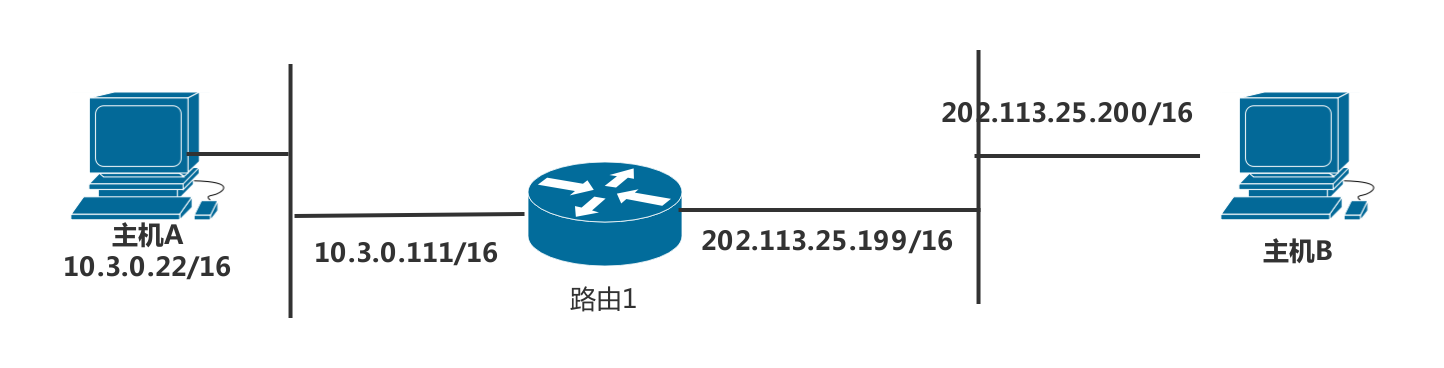
\includegraphics[width=0.6\textwidth]{互联网拓扑图}
	\caption{虚拟机互联网拓扑图结构 \label{fig:tuopu}}
\end{figure}


设置虚拟机的IP地址的步骤为:选择“路由与远程访问”的本地接口,选择“常规”,在界面中可以看到两个本地连接,分别对应虚拟机的两个网卡,在本次实验中,两台终端机器只需要使用一张网卡一个IP即可,NAT服务器需要为两张网卡分别配置一个IP,一个作为内网的网关,一个作为外网的网关。需要注意的是,作为终端机使用的主机A和主机B需要在设置IP地址的同时,设置好对应的默认路由(即为NAT服务器对应的网关IP)。主机A与主机B的IP地址配置如\figref{fig:1}所示,NAT服务器的两张网卡的IP设置如\figref{fig:2}所示。

\begin{figure}[htbp]
	\begin{minipage}[t]{0.5\textwidth}
		\centering
		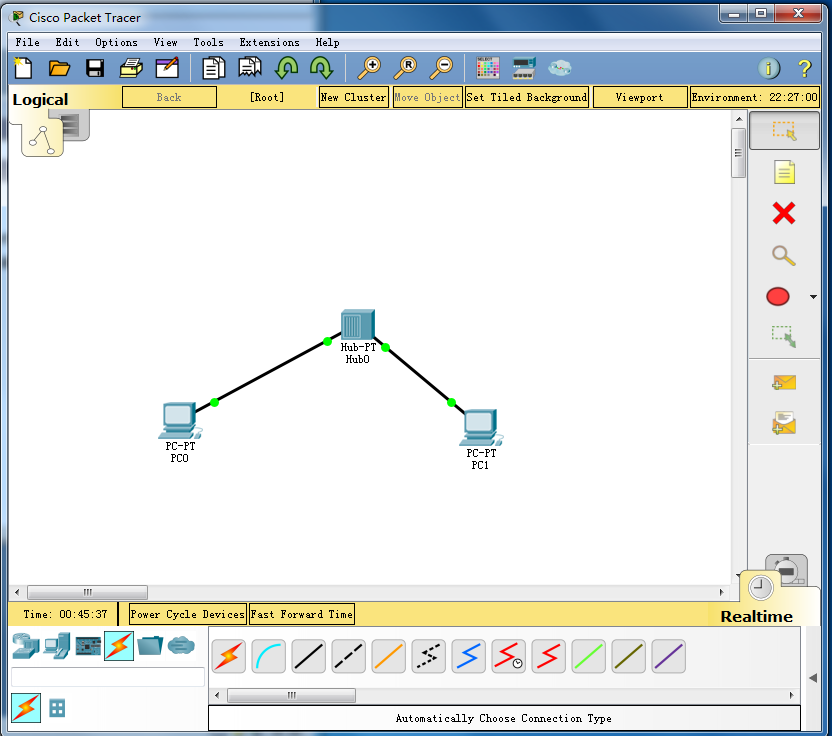
\includegraphics[width=0.7\textwidth]{1}
	\end{minipage}
	\begin{minipage}[t]{0.5\textwidth}
		\centering
		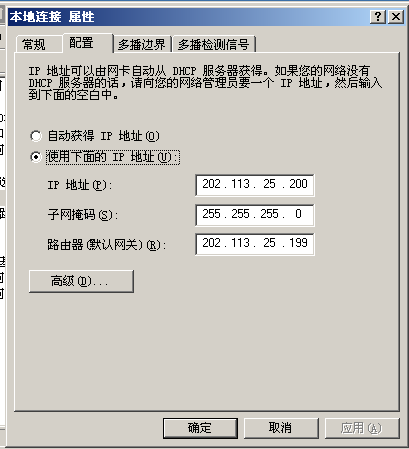
\includegraphics[width=0.7\textwidth]{11}
	\end{minipage}
		\caption{主机A与主机B的IP地址及默认网关设置 \label{fig:1}}
\end{figure}

\begin{figure}[htbp]
	\begin{minipage}[t]{0.5\textwidth}
		\centering
		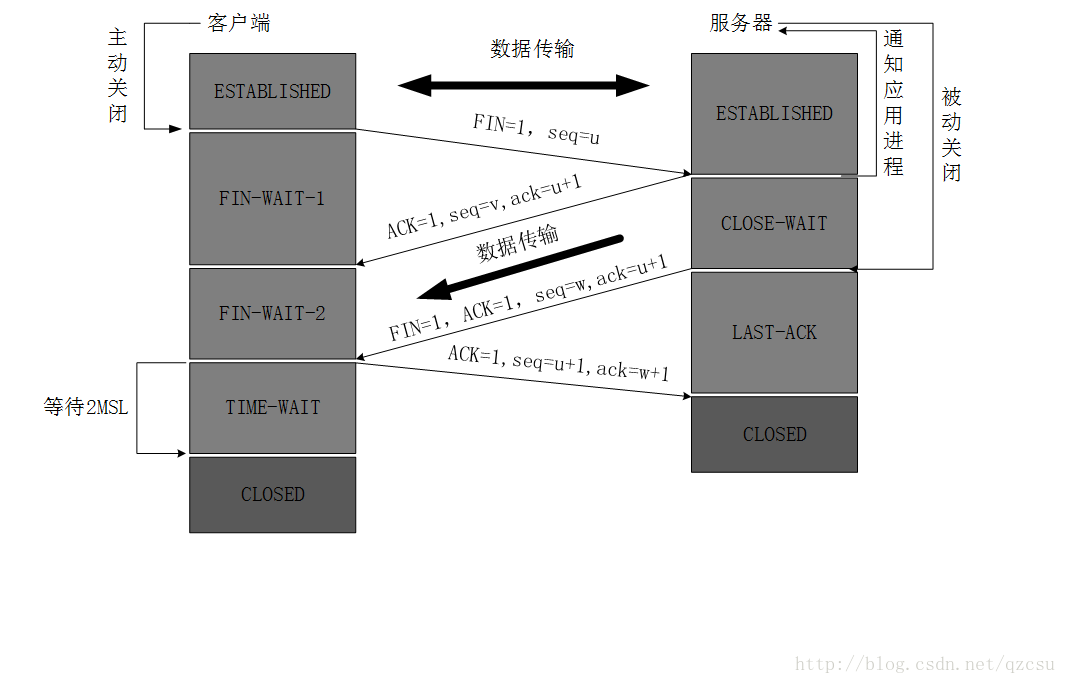
\includegraphics[width=0.7\textwidth]{2}
	\end{minipage}
	\begin{minipage}[t]{0.5\textwidth}
		\centering
		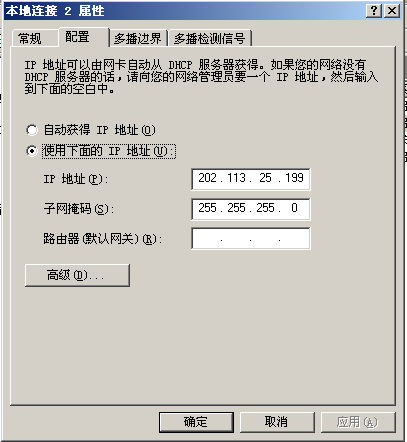
\includegraphics[width=0.7\textwidth]{3}
	\end{minipage}
		\caption{NAT网卡的IP地址配置 \label{fig:2}}
\end{figure}

\subsubsection{NAT转换配置}
配置好虚拟主机的IP地址之后,开始配置NAT服务器的NAT接口,通过“路由与远程访问”程序实现,在这里以后一种方式说明,“程序与远程访问”界面如\figref{fig:jiemian}所示:

\begin{figure}[htbp]
	\centering
	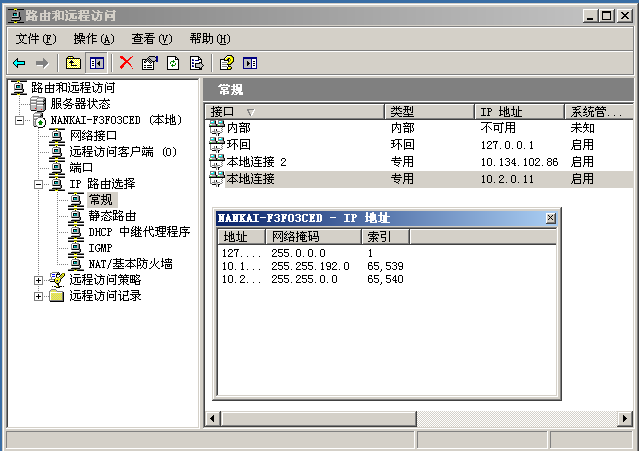
\includegraphics[width=0.6\textwidth]{ipset3}
	\caption{程序与远程访问界面截图演示\label{fig:jiemian}}
\end{figure}


从截图\figref{fig:jiemian}可以看到NAT/基本防火墙的选项,打开后在空白界面右键选择“新建接口”即可选择为相应的网卡连接添加NAT接口,新建接口的窗口界面如\figref{fig:5}所示,在建立内网的NAT接口时选择专有网络接口,在建立外网NAT转换时选择“公用网络到Internet”以及“在此接口启用NAT”。
\begin{figure}[htbp]
		\centering
		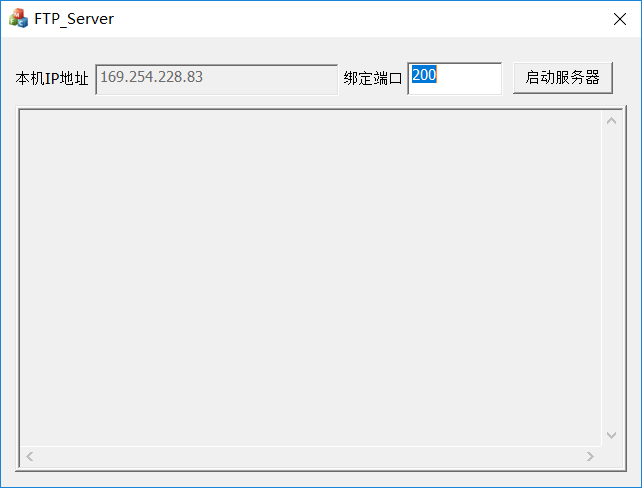
\includegraphics[width=0.6\textwidth]{5}
			\caption{建立NAT接口配置选项 \label{fig:5}}
\end{figure}

为\figref{fig:tuopu}中的NAT服务器的两张网卡分别添加NAT后的“程序与远程访问”界面\figref{fig:3}所示:

\begin{figure}[htbp]
	\centering
	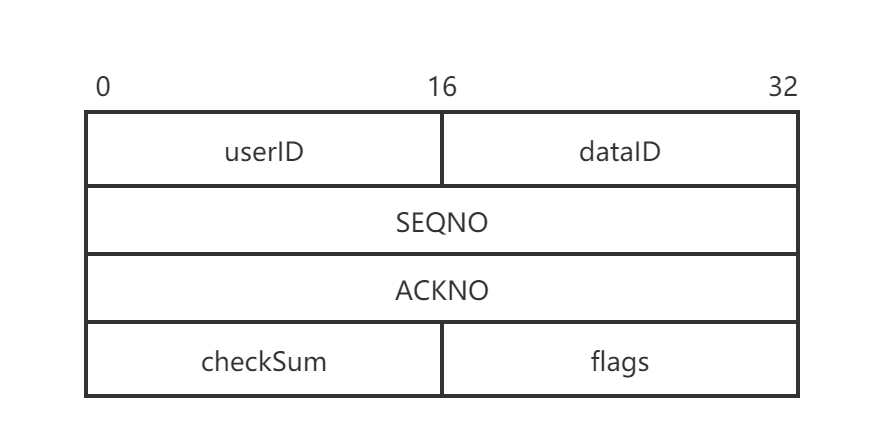
\includegraphics[width=0.6\textwidth]{4}
	\caption{NAT配置界面\label{fig:3}}
\end{figure}

\subsubsection{NAT穿透}
由于本次实验要求从外网能够访问内网的web服务器,因此需要将内网中的主机A作为web服务器供外网进行访问,正常情况下外网是无法获取内网IP进行访问的,但是可以通过穿透NAT的方式将内网的IP和对外的公网IP地址做一个映射关系实现外网终端对内网web服务器的访问,实现方式为在对外公网NAT接口上添加Web服务接口,将内网的web服务器IP和公网IP进行端口映射,实现静态NAT的效果,如\figref{fig:6}、\figref{fig:7}所示,选择web服务器,并将专有地址设置为内网web服务器终端的IP地址如\figref{fig:7}所示。

\begin{figure}[htbp]
	\begin{minipage}[t]{0.5\textwidth}
		\centering
		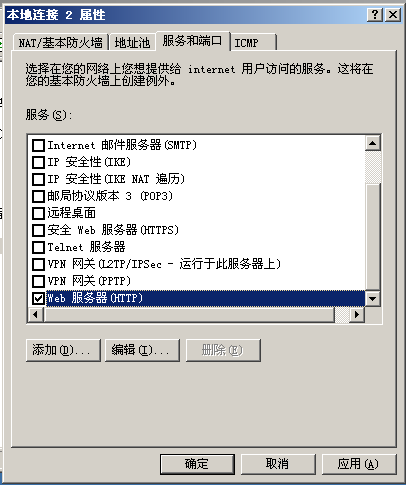
\includegraphics[width=0.7\textwidth]{6}
			\caption{服务与端口界面 \label{fig:6}}
	\end{minipage}
	\begin{minipage}[t]{0.5\textwidth}
		\centering
		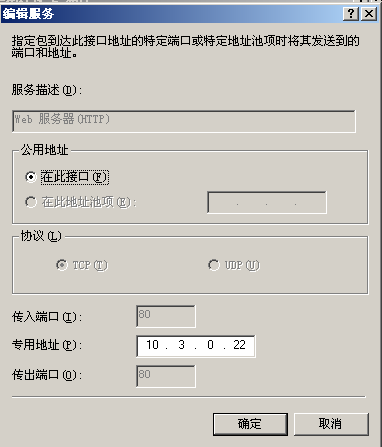
\includegraphics[width=0.7\textwidth]{7}
			\caption{web服务器服务设置 \label{fig:7}}
	\end{minipage}

\end{figure}

\subsubsection{连通性测试}
在配置好NAT服务器和web服务终端之后,需要进行连通性测试,在本实验中,内网的终端能够访问外网的机器,同时外网的机器也能够访问内网的特定web服务器终端,在下面主要展示主机A、B之间的连通性测试,连通性测试结果如\figref{fig:8}所示,web服务器访问测试结果如\figref{fig:A}、\figref{fig:B}所示:
\begin{figure}[htbp]
	\centering
	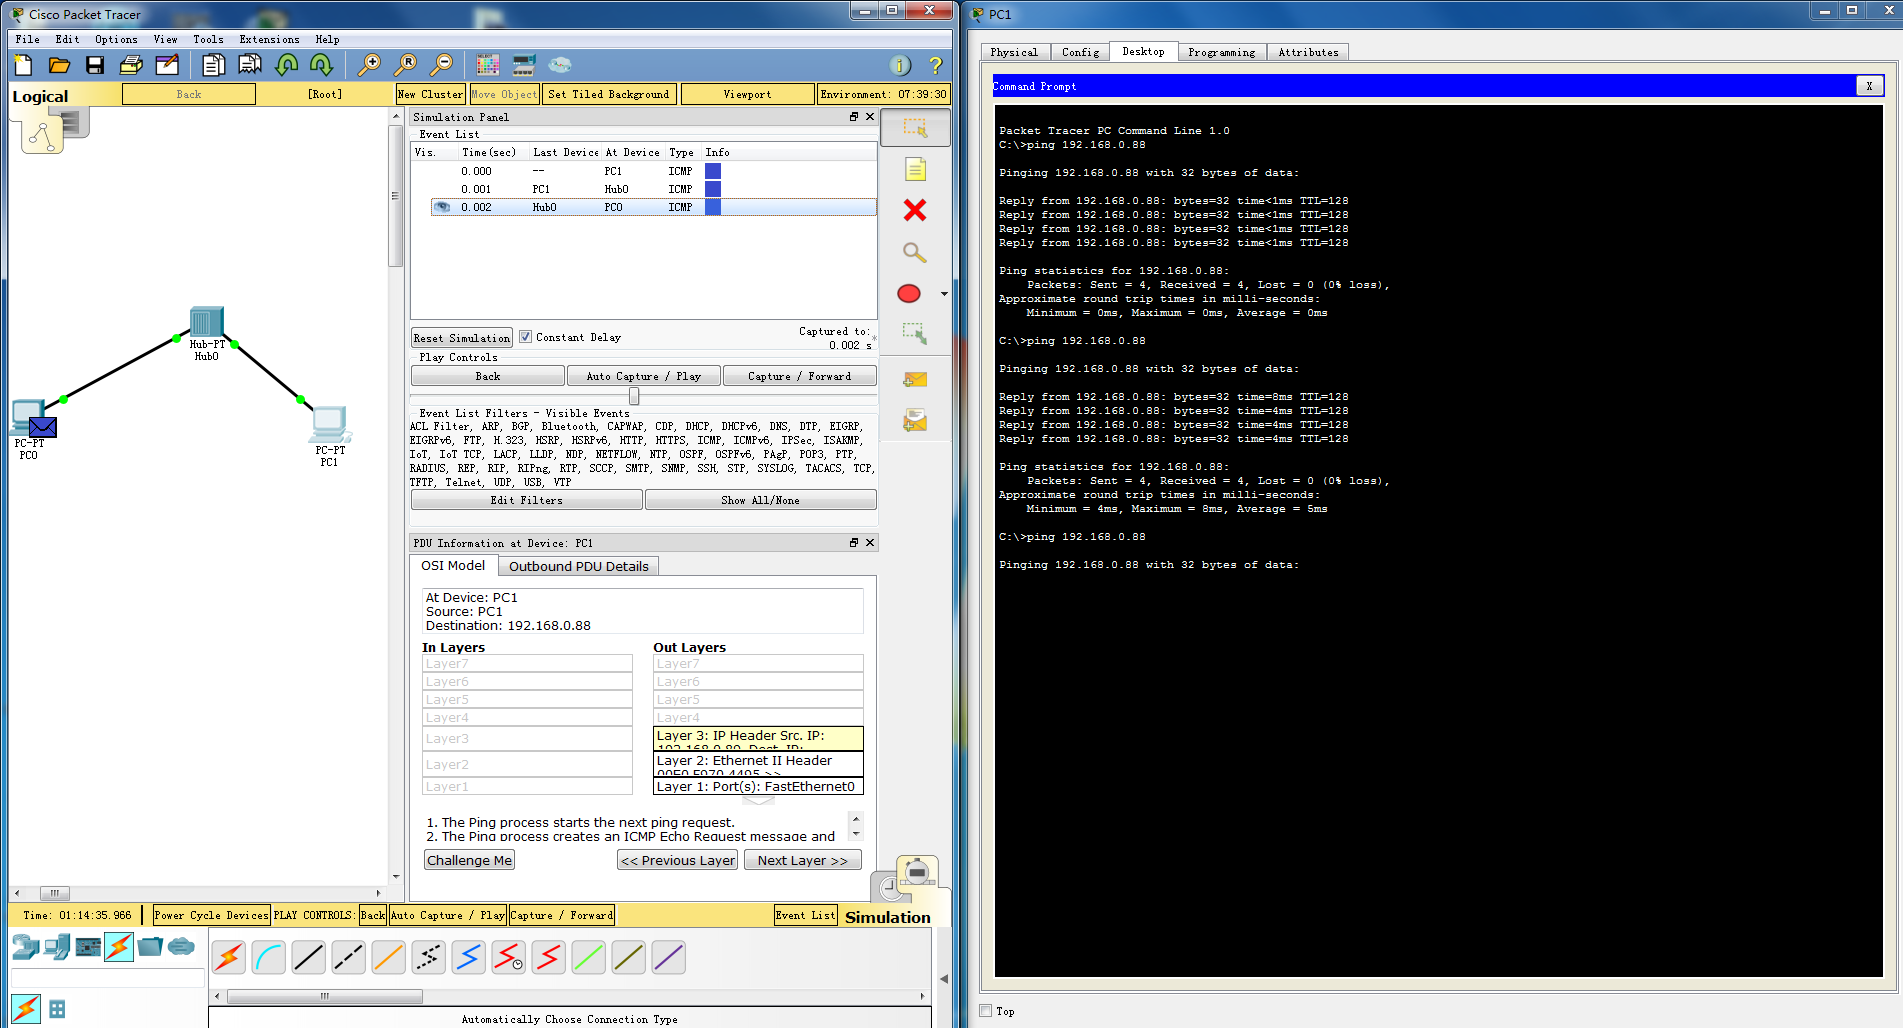
\includegraphics[width=0.4\textwidth]{8}
	\caption{主机Aping主机B的结果截图\label{fig:8}}
\end{figure}

\begin{figure}[htbp]
	\begin{minipage}[t]{0.5\textwidth}
		\centering
		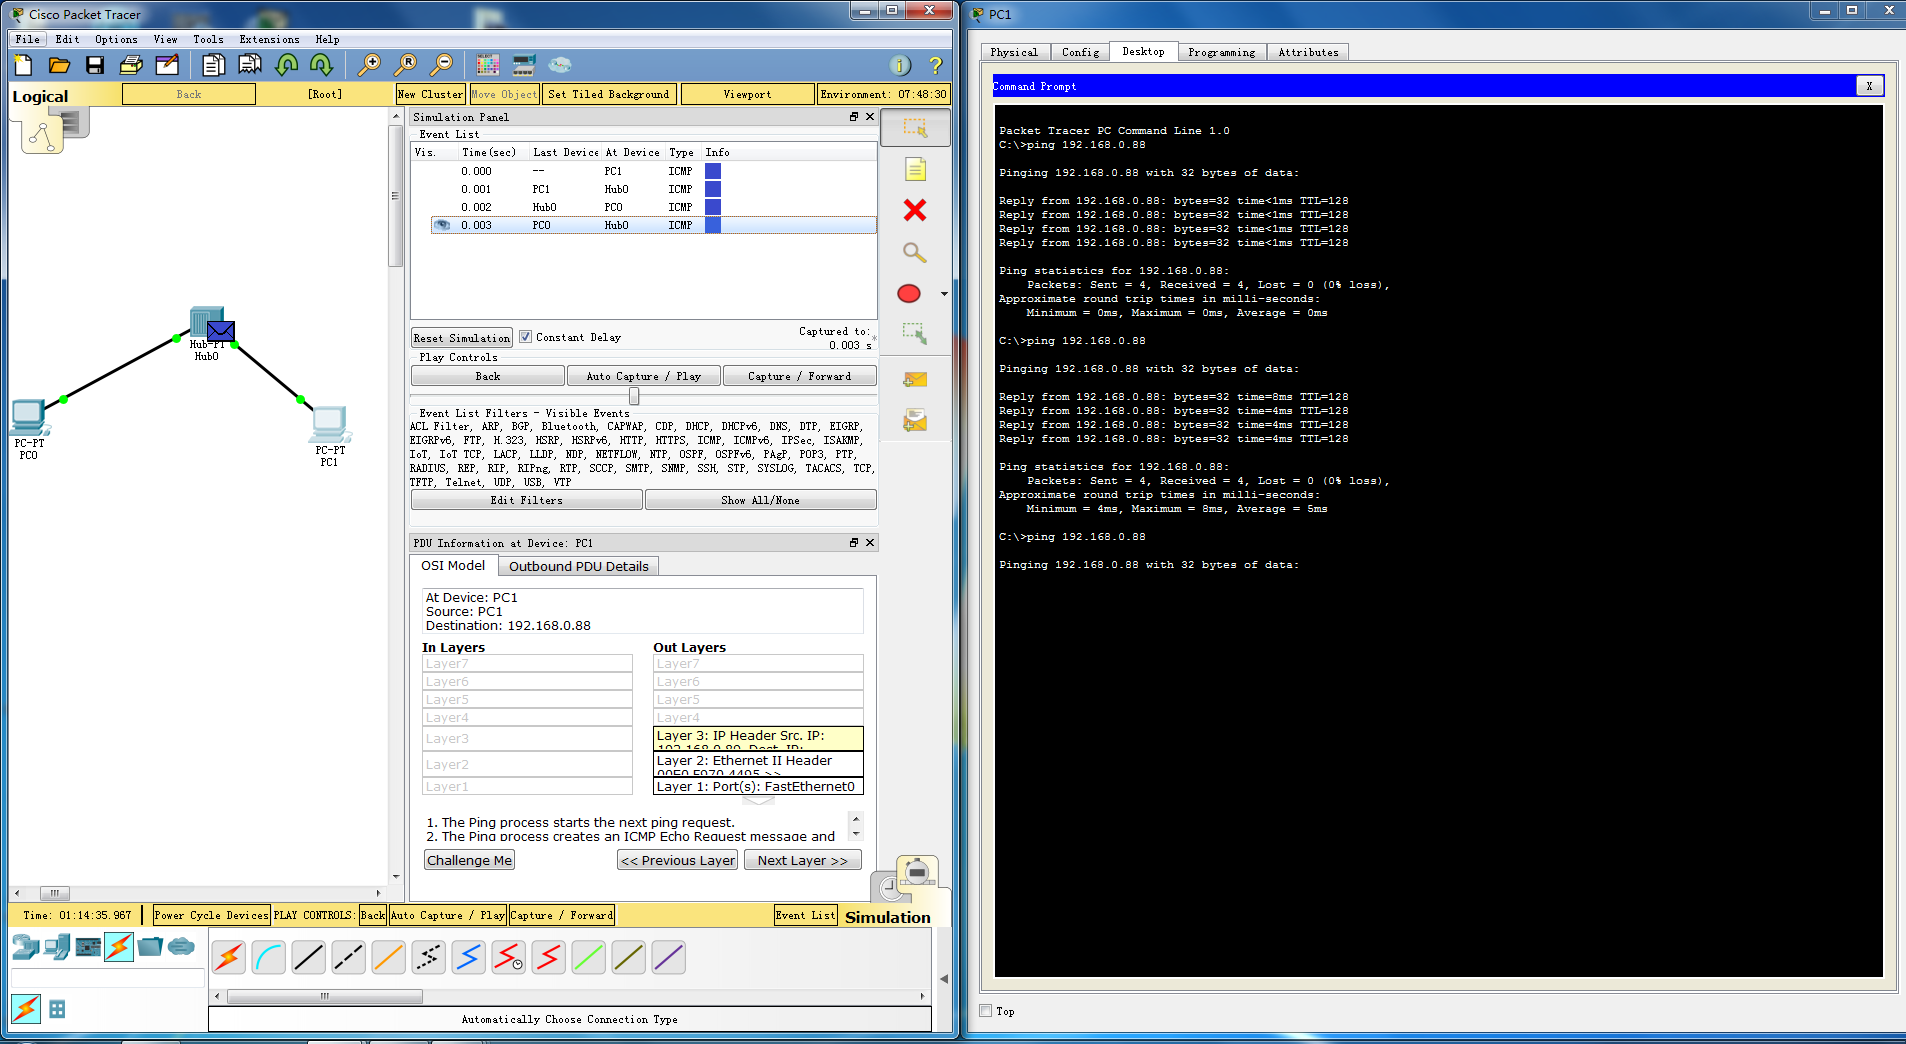
\includegraphics[width=0.7\textwidth]{9}
		\caption{主机A访问外网web服务器\label{fig:A}}
	\end{minipage}
	\begin{minipage}[t]{0.5\textwidth}
		\centering
		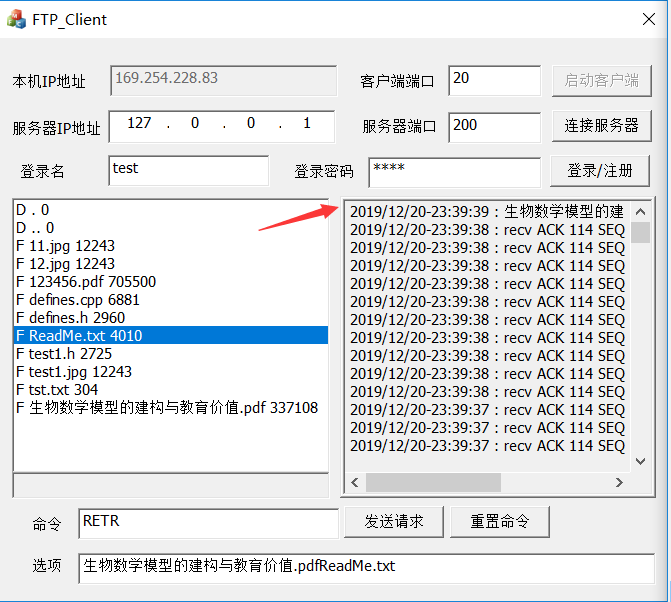
\includegraphics[width=0.7\textwidth]{12}
		\caption{主机B访问内网web服务器 \label{fig:B}}
	\end{minipage}
\end{figure}

\subsection{仿真环境NAT配置}
\subsubsection{IP地址和设备配置}
与虚拟机环境类似,仿真环境下的配置步骤基本没有区别,都是先进行IP地址的配置,然后配置NAT议,\figref{fig:11}显示的是网络拓扑图以及相关接口的IP地址配置。
\begin{figure}[htbp]
	\centering
	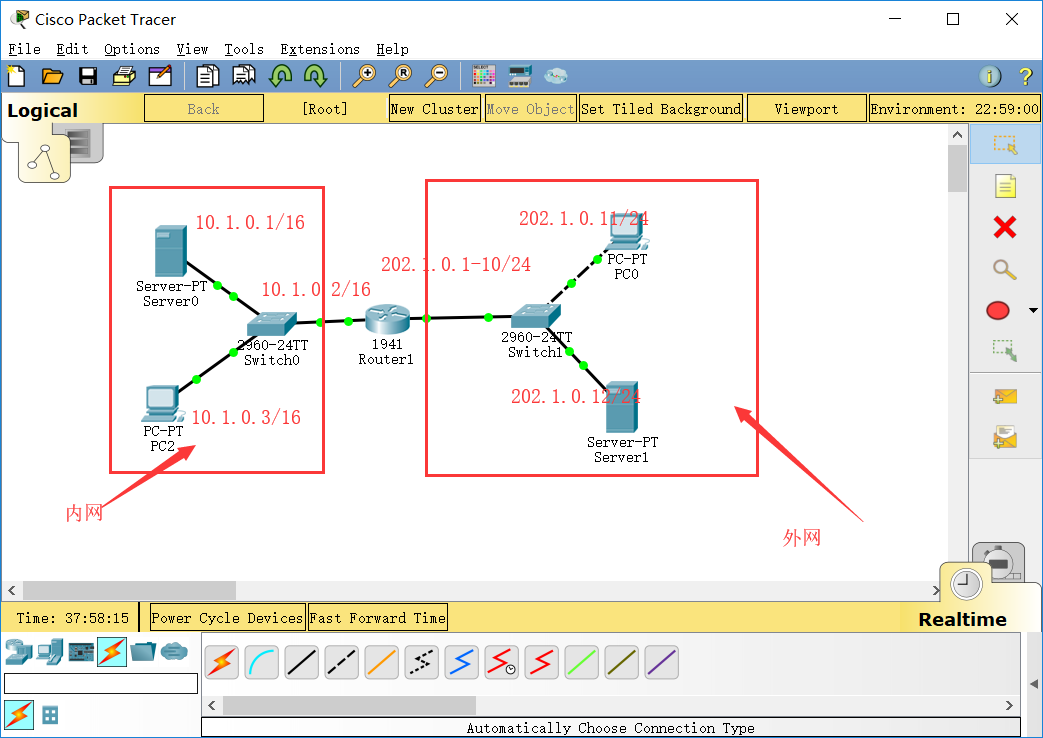
\includegraphics[width=0.6\textwidth]{17}
	\caption{仿真环境互联网拓扑图结构 \label{fig:11}}
\end{figure}

按照网络拓扑图中的IP地址配置好了主机的IP地址之后,进一步可以配置NAT,在仿真环境下的路由配置主要通过路由器的CLI中的命令进行NAT的配置。配置NAT的命令主要是IP nat pool 、 access-list 、ip nat inside  list  LabelID pool PoolName overload,由于需要从外网访问内网web服务器,所以需要配置静态的NAT,配置过程如下所示:

\begin{lstlisting}
Router>enable 
Router#config terminal
Enter configuration commands, one per line.  End with CNTL/Z.
Router(config)#ip nat inside source static tcp 10.1.0.1 80 202.1.0.1 80
Router(config)#exit
Router#
%SYS-5-CONFIG_I: Configured from console by console

Router#exit
\end{lstlisting}

最终生成的NAT映射表如下所示,其中第二条为静态NAT映射。
\begin{lstlisting}
Router>show ip nat translations
Pro  Inside global     Inside local       Outside local      Outside global
tcp 202.1.0.1:1097     10.1.0.3:1097      202.1.0.12:80      202.1.0.12:80
tcp 202.1.0.1:80       10.1.0.1:80        ---                ---
tcp 202.1.0.1:80       10.1.0.1:80        202.1.0.11:1170    202.1.0.11:1170
\end{lstlisting}

\subsubsection{测试结果截图}
测试web服务器的访问截图如\figref{fig:14}、\figref{fig:15}所示,由于修改过web服务器的默认页面,所以可以通过查看页面内容判断访问的web服务器是哪一个。
\begin{figure}[htbp]
		\centering
		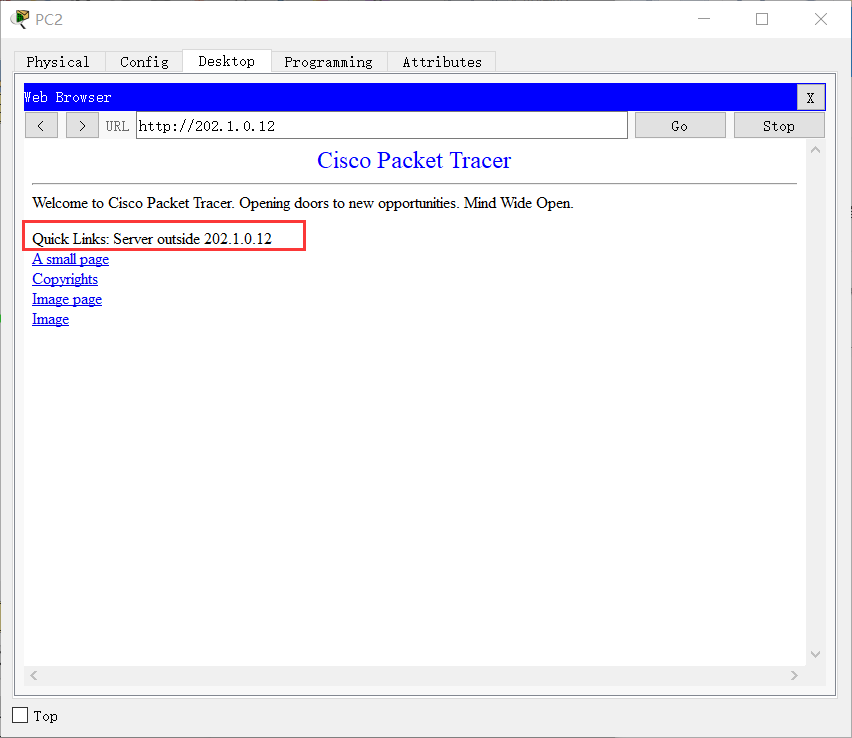
\includegraphics[width=0.6\textwidth]{18}
	\caption{内网访问外网web服务器\label{fig:14}}
\end{figure}

\begin{figure}[htbp]
	\centering
	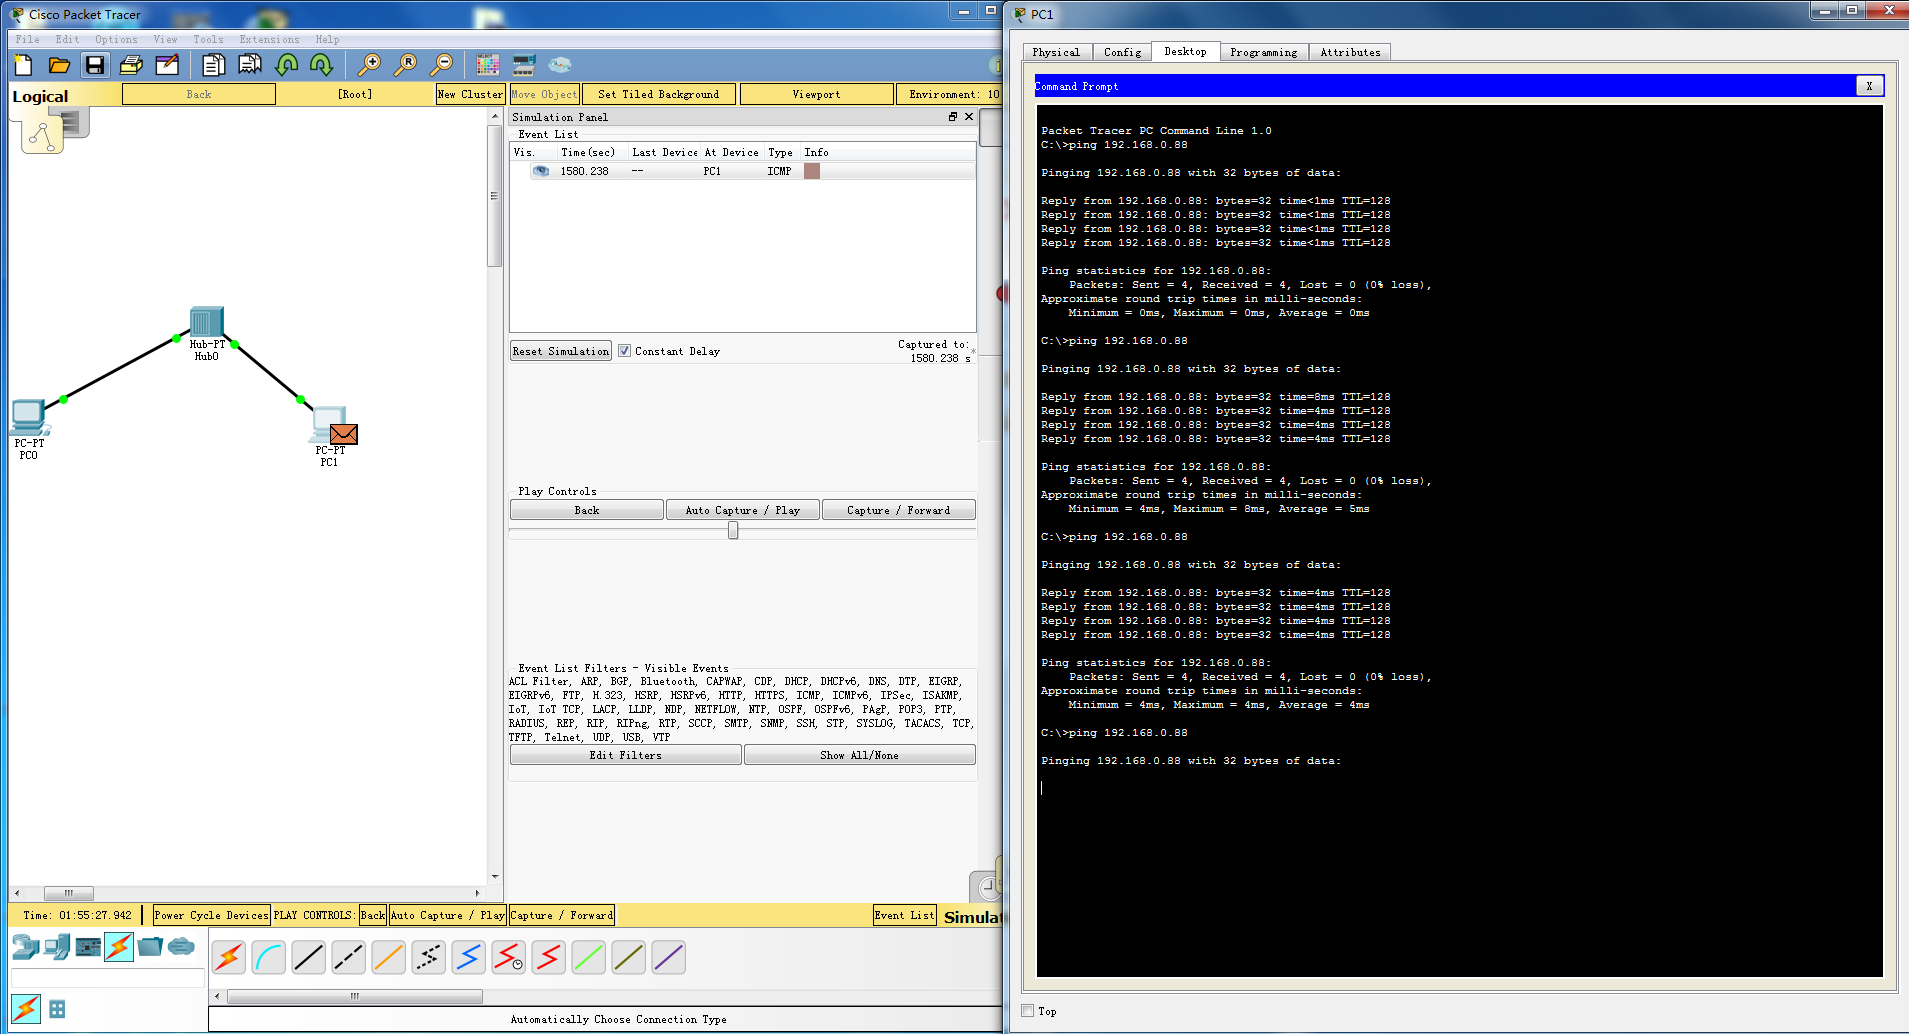
\includegraphics[width=0.6\textwidth]{19}
	\caption{外网访问内网web服务器 \label{fig:15}}
\end{figure}
\newpage
\section{总结与思考}
通过这次在三台虚拟机上进行NAT的配置以及在仿真环境下配置NAT并实现了从外网访问内网web服务器,进一步了解到了关于NAT的相关知识,深入理解了网络地址转换工作的基本原理和配置NAT的相关工作,能够理解网络地址映射形成的过程和网络地址转换在网络通信中的巨大作用。在这次实验的过程中发现,网络地址转换在很大程度上确实降低了对IP地址的数量上的要求,但是仍然让类似于服务器通信之类的网络服务变得不太方便,但是在另一方面NAT的存在对网络安全有一定的作用,起到的基本的网络防火墙功能。


% 如果想修改参考文献样式(非国标),请把下行取消注释,并换成合适的样式(比如 unsrt,plain 样式)。
%\bibliographystyle{aer}
%\bibliography{wpref}

\end{document}
